\documentclass[]{article}

\usepackage[spanish]{babel} % Configurar el idioma a español
\usepackage[utf8]{inputenc} % Permitir caracteres especiales como acentos y ñ
\usepackage[T1]{fontenc}    % Mejor codificación para caracteres en español
\usepackage{authblk} % Paquete para filiaciones institucionales
\usepackage{geometry} % Paquete para configurar márgenes
\usepackage{multicol} % Paquete para columnas múltiples
\usepackage{graphicx} % Paquete para incluir imágenes
\usepackage{lipsum}   % Paquete para texto de ejemplo
\usepackage[numbers]{natbib} % Paquete para citas bibliográficas

% Configuración de márgenes
\geometry{
	top=2cm,    % Margen superior
	bottom=3cm, % Margen inferior
	left=2cm,   % Margen izquierdo
	right=2cm   % Margen derecho
}

\bibliographystyle{plain} % Estilo de bibliografía

\title{Desarrollo de un dispositivo de adquisición vectorcardiográfica con corrección de alteraciones posturales abruptas}

\author[1]{Autor 1}
\author[1]{Autor 2}
\author[1]{Autor 3}
\author[1,2]{Pablo Daniel Cruces\thanks{Correspondencia a: Pablo Daniel Cruces, Paseo Colón 850, IIBM 4° Piso, CABA (C1063ACV), Argentina; pcruces@fi.uba.ar; (54-11) 528 - 50927.}} % Se marca la correspondencia con \thanks
\affil[1]{Laboratorio Abierto de Bioingeniería (BiLAB), Departamento de Bioingeniería, Facultad de Ingeniería, UBA, Paseo Colón 850 (C1063ACV), CABA, Argentina}
\affil[2]{Instituto Argentino de Matemática 'Alberto P. Calderón', CONICET, Saavedra 15 (C1083ACA), Buenos Aires, Argentina\newline}

\date{}

\begin{document}

\maketitle

\begin{abstract}

Las patologías cardiovasculares representan un tercio de las defunciones a nivel nacional y mundial. El diagnóstico concluyente suele ser en etapas avanzadas de la enfermedad cuando ya se presentan síntomas graves y en muchos casos, no reversibles. En este trabajo, se presenta un dispositivo de adquisición de tres señales electrocardiográficas ortogonales con un sensor de velocidad angular y aceleración lineal incorporado. Un algoritmo permite adaptar los bucles eléctricos cardíacos a la posición del cuerpo y corregir alteraciones que podrían dar falsos positivos en el diagnóstico de isquemia. El desarrollo de dispositivos de bajo costo no invasivos para la medición de las diversas variables fisiológicas del sistema cardiovascular puede proporcionar una herramienta para la detección temprana de anomalías físicas. Estos dispositivos podrían aplicarse a diagnósticos de rutina en salas de primeros auxilios y hospitales alejados de las ciudades permitiendo un alcance al total de la población.

\end{abstract}

\vspace{20pt}

\begin{multicols}{2}
\section{Introducción}
Introducción detallada del estado del arte, los objetivos del trabajo, el alcance y las implicancias a nivel social.

\lipsum[1] % Texto de ejemplo



\section{Materiales y Métodos}
En la Fig. \ref{Fig_Esquema} se muestra el esquema de proceso. La configuración de electrodos se corresponde con el sistema EASI y se emplea un método lineal para obtener las derivaciones XYZ de Frank \cite{Feild2002}.

\end{multicols}
\begin{figure}[ht]
\centering
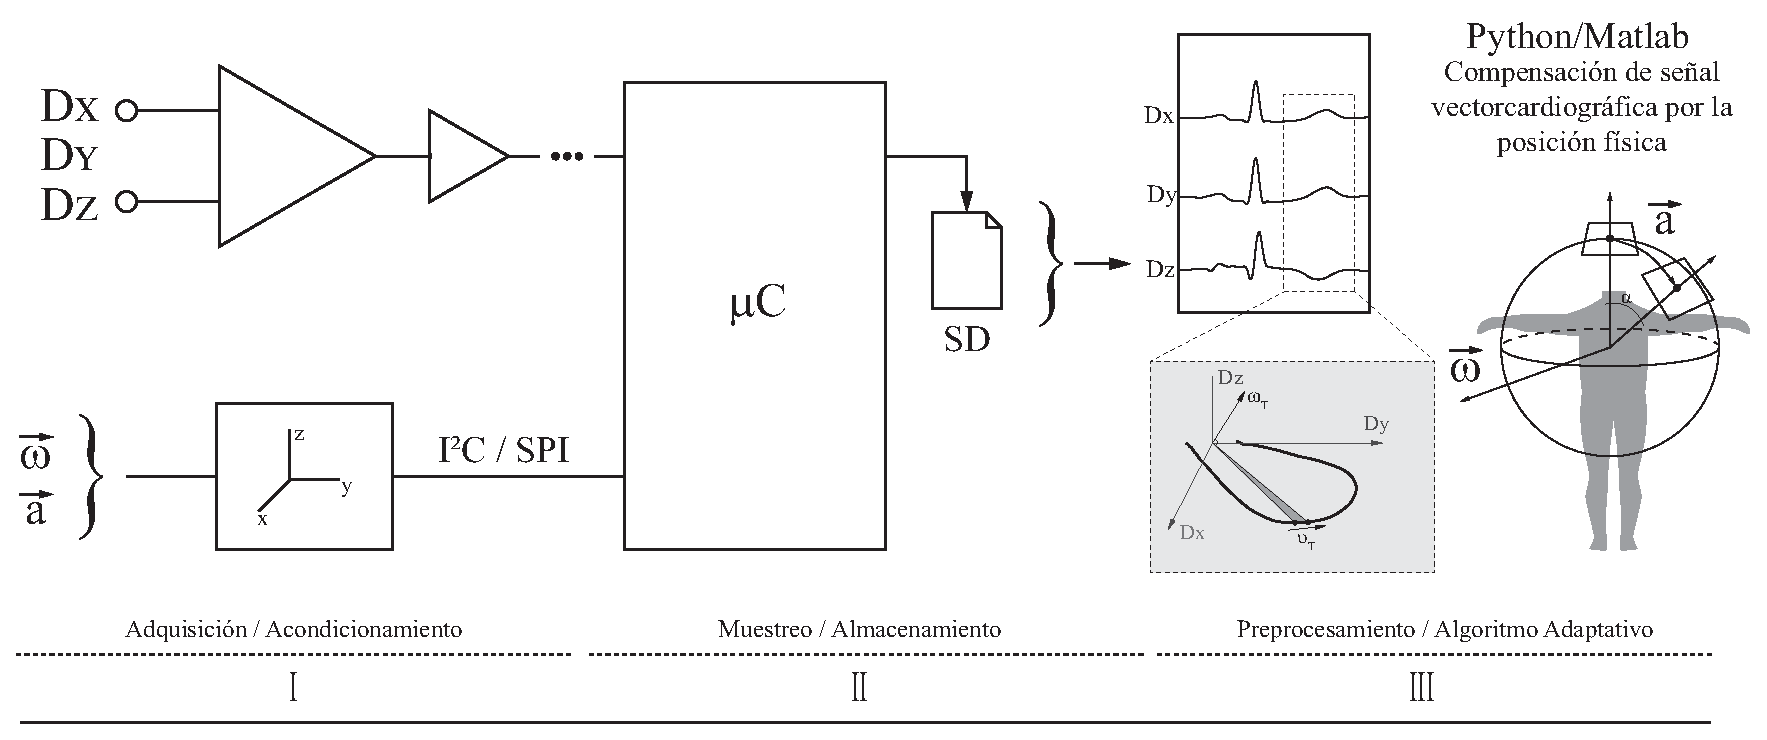
\includegraphics[width=\textwidth]{Imags/Esquema.eps} 
\caption{Esquema del prototipo.}
\label{Fig_Esquema}
\end{figure}
\begin{multicols}{2}

\lipsum[2-3] % Más texto de ejemplo

\end{multicols}

\bibliography{refs} % Vincular a refs.bib

\end{document}
